%=============================================%
\begin{frame}
	\large
	\texttt{Account Types}
	\begin{figure}
		\centering
		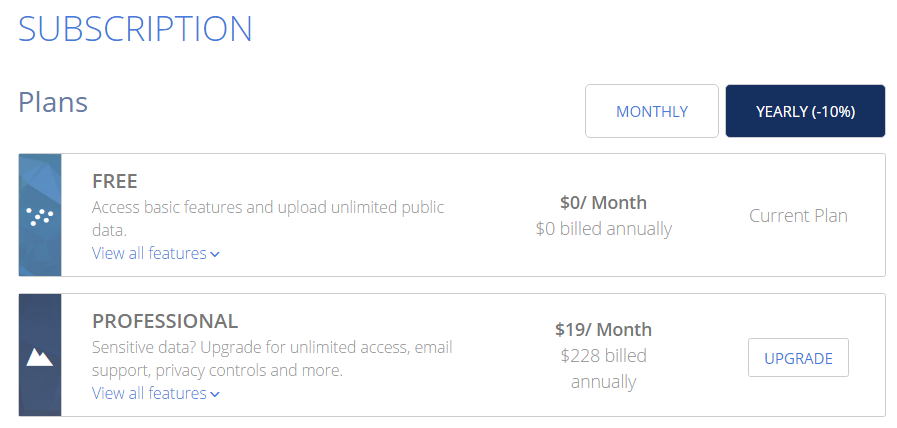
\includegraphics[width=01.1\linewidth]{plotlysubscription}
	\end{figure}
	
\end{frame}
%=============================================%
\begin{frame}
	\large
	\texttt{Industry}
	\begin{figure}
		\centering
		
\includegraphics[width=01.1\linewidth]{plotlyindustry}
	\end{figure}
	
\end{frame}


%==============================================%
\begin{frame}
	\begin{figure}
\centering

\includegraphics[width=1.3\linewidth]{jupyter}
\end{figure}
\end{frame}
%==============================================%
\begin{frame}
\texttt{Installation}\\
To install Plotly's python package, use the package manager pip inside your terminal.
If you don't have pip installed on your machine, click here for pip's installation instructions. 
\end{frame}
%===========================================================%
%=======================%
\begin{frame}[fragile]
	\large
\begin{framed}
	\begin{verbatim}
	$ pip install plotly 
	or 
	$ sudo pip install plotly 
	
	Plotly's Python package is updated frequently! To upgrade, run: 
	
	$ pip install plotly --upgrade
	\end{verbatim}
\end{framed}
\end{frame}